\chapter{Appendix B -- OpenDroneMap Tipps}

\section{Kameraprofil erstellen}

\label{ch:odm-camera-profile}

Damit OpenDroneMap die übergebenen Bilder richtig verarbeiten kann, benötigt die
Software Informationen über die Abmessungen des Kamera-Sensors. Diese
Informationen sind für viele Kameramodelle bereits in OpenDroneMap registriert.

Falls ein Kameramodell noch fehlt, wird die folgende Fehlermeldungen erzeugt:

\begin{verbatim}
no CCD width or focal length found for DSC05399.JPG \
  - camera: "SONY ILCE-5100"
found no usable images - quitting
\end{verbatim}

Wie aus der Meldung ersichtlich, wurde das Bild mit einer SONY ILCE-5100 Kamera
erstellt, welche OpenDroneMap noch nicht bekannt ist. Eine kurze Google-Suche ergibt,
dass die SONY ILCE-5100 identisch ist mit der SONY A5100.

Die Sensorgrösse einer Kamera findet man relativ einfach auf der Website
\url{dpreview.com}. Die SONY A5100 ist vertreten:
\url{http://www.dpreview.com/products/sony/slrs/sony_a5100}

In der "<Quick Specs"> Liste wird unter "<Sensor size"> die Sensorgrösse
aufgelistet:

\begin{figure}[H]
	\centering
	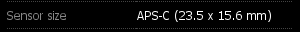
\includegraphics[width=3in]{images/sensor.png}
	\caption{Sensorgrösse SONY A5100}
\end{figure}

Den grösseren der zwei Werte muss man nun im OpenDroneMap Sourcecode in die
Datei \texttt{ccd\_defs.json} eintragen:

\begin{minted}[bgcolor=tango-bg,frame=lines,framesep=2mm,samepage=true,fontsize=\footnotesize]{json} 
{
  // ...
  "SONY ILCE-5100": 23.5,
  // ...
}
\end{minted}

Nun OpenDroneMap erneut starten und die Fehlermeldung sollte verschwinden.
